La figure \ref{fig:supply} récapitule la chaîne d'approvisionnement de certaines technologies bas carbone qui utilisent les matériaux que nous avons étudiés dans la sous-section précédente. Elle met en évidence le fait que la Chine est présente sur l'ensemble de la chaîne, ce qui peut lui procurer une forme de suprématie économique et la mettre en bonne voix pour asseoir un leadership sur le secteur des technologies de la transition énergétique. 
\smallbreak
En ce qui concerne l'amont de la chaîne, le raffinage apporte plus de valeur ajoutée et des emplois plus qualifiés que l'extraction. Cela peut amener des pays détenteurs de réserves à développer des capacités de transformation afin de ne pas tomber dans la malédiction des ressources, ainsi que pour avoir plus de poids face aux puissances dépendantes d'importations de métaux, comme les Etats-Unis et l'Union européenne. C'est notamment le cas en Indonésie, qui a décrété à plusieurs reprises des embargos sur ses exportations de minerais bruts (voir encadré \hyperref[Indonesia]{\textit{L'Indonésie et le nickel : existe-t-il un risque de cartellisation ?}}).
\smallbreak
Face aux risques de ruptures d'approvisionnement, en plus de la diversification des fournisseurs, les pays dépendants de ces métaux pour leur transition énergétique peuvent trouver un intérêt à relocaliser l'amont de la chaîne. De plus, avoir la main sur l'ensemble des étapes implique plus de visibilité et de transparence sur le respect des normes environnementales et le droit du travail. Seulement, du fait de plus faibles réserves, seuls de petits volumes de production pourraient être tirés de ces mines et raffineries relocalisées. Cela, de même que les normes environnementales et humaines plus sévères, rendent ces solutions peu compétitives et tributaires de prix hauts pour être rentables. Par exemple, à la suite de l'embargo non-officiel de la Chine sur les terres rares (voir encadré \hyperref[Chine]{\textit{Les terres rares chinoises : une arme économique et géopolitique}}), les Etats-Unis ont fait rouvrir la mine de Mountain Pass en 2012. Mais la prépondérance de la RPC dans ce secteur lui a permis de faire jouer les prix des terres rares à la baisse, entraînant une perte de valeur de 20\% pour les actions de Mollycorp, l'entreprise alors propriétaire du site (\cite{niquet_chine_2011}). Cette dernière a déposé bilan en 2015 (\cite{hsu_molycorp_2015}).

\begin{figure}[!b]
    \centering
    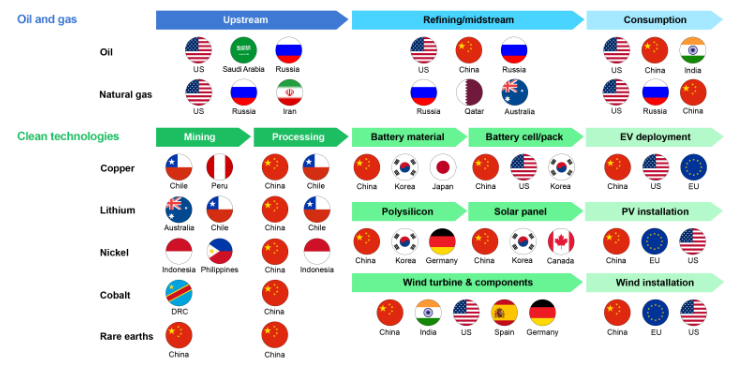
\includegraphics[width=0.8\textwidth]{Images/02 appro/SC metaux.png}
    \caption{Chaînes d'approvisionnement indicatives du pétrole et du gaz et de certaines technologies d'énergie propre. Source : \cite{iea_role_2021}}
    \label{fig:supply}
\end{figure}

\begin{center}
    \boxput*(0,1){
        \colorbox{white}{L'Indonésie et le nickel : existe-t-il un risque de cartellisation ?}
    }{
    \setlength{\fboxsep}{15pt}
    \fbox{\begin{minipage}{14cm} 
L'Indonésie a, à plusieurs reprises, mis en place des politiques d'interdiction d'exportation de minerais non transformés. La première a eu lieu entre 2014 et 2017, et la seconde a commencé en 2020 et se poursuit aujourd'hui. Cette dernière concerne pour l'instant seulement le nickel brut, mais le président Jokowi a annoncé sa possible extension à la bauxite, l'étain et le cuivre. Pour cet embargo, l'Organisation Mondiale du Commerce a condamné l'Indonésie fin 2022 à la suite d'une plainte de l'Union européenne, décision contre laquelle le pays asiatique compte faire appel.\smallbreak
L'objectif derrière ces politiques est d'encourager les investissements directs étrangers vers des fonderies ou des usines de raffinage sur le sol indonésien. Ainsi, le pays espère capter plus de valeur ajoutée, et créer plus d'emplois locaux. Mais ces embargos successifs ont également encouragé les investissements dans les projets miniers dans d'autres pays, ce qui pourrait affaiblir la position de l'Indonésie sur le long terme.\smallbreak
Au-delà des considérations économiques, les restrictions indiquent aussi une volonté géopolitique d'affichage de puissance : il s'agit ici de montrer que le pays a la capacité d'influence pour disrupter le cours du nickel. Cela s'est en outre traduit par une déclaration faite par le ministre de l’Investissement Bahlil Lahadalia dans le Financial Times en octobre 2022 : l'Indonésie étudie la possibilité de créer un cartel, similaire à l'Organisation des Pays Producteurs de Pétrole (OPEP), pour les principaux producteurs de métaux des batteries.\smallbreak
Seulement, on peut s'interroger sur la vraisemblance du risque de cartellisation pour les métaux. Si l'OPEP a une telle importance géopolitique, c'est notamment grâce à la vague de nationalisation de la production pétrolière par ses pays fondateurs, qui a transféré le pouvoir d'influence des majors vers les gouvernements. Or, dans le cas du nickel, rien qu'en Indonésie, pourtant porteuse de l'initiative, les entreprises étrangères constituent une grande part de la production, dont la brésilienne Vale qui est même un des acteurs majeurs du secteur minier indonésien.

\textit{Sources : \cite{hache_metaux_2022},\cite{strangio_indonesia_2022}}

    \end{minipage}}
    }
\end{center}
\label{Indonesia}
~\\